\documentclass[pra,showkeys,twocolumn,showpacs]{revtex4-1}
\usepackage{amsmath}
\usepackage{amsfonts}
\usepackage{amssymb}
\usepackage{array}
\usepackage{color}
\usepackage{soul}
%\usepackage{floatflt}
\usepackage{graphicx}
\DeclareMathOperator{\tr}{Tr}
\newcommand*{\eq}[1]{(\ref{#1})}
\newcommand*{\eqs}[2]{(\ref{#1})--(\ref{#2})}
\newcommand{\exi}{\tr{\{e^{-\frac\beta2\sum_k\lambda_k\gamma_k^\dag\gamma_k}\}}}
\renewcommand{\l}{\left(}
\renewcommand{\r}{\right)}

\usepackage[inline]{enumitem} % inline enumeration

\begin{document}
\title{Hybrid quantum-classical unsupervised data clustering on the basis of Self-Organizing Feature Map}

\author{I.~D.~Lazarev} 
\affiliation{Institute of Problems of Chemical Physics of Russian Academy of Sciences, Acad. Semenov av. 1, Chernogolovka, Moscow Region, Russia, 142432}
\affiliation{ Faculty of Fundamental Physical-Chemical Engineering, Lomonosov Moscow State University, GSP-1, Moscow, Russia 119991}

\author{Marek Narozniak}
\affiliation{New York University Shanghai, 1555 Century Ave, Pudong, Shanghai 200122, China}
\affiliation{Department of Physics, New York University, New York, NY, 10003, USA.}

\author{Tim Byrnes}
\affiliation{New York University Shanghai, 1555 Century Ave, Pudong, Shanghai 200122, China}
\affiliation{State Key Laboratory of Precision Spectroscopy, School of Physical and Material Sciences, East China Normal University, Shanghai 200062, China}
\affiliation{NYU-ECNU Institute of Physics at NYU Shanghai, 3663 Zhongshan Road North, Shanghai 200062, China}
\affiliation{National Institute of Informatics, 2-1-2 Hitotsubashi, Chiyoda-ku, Tokyo 101-8430, Japan}
\affiliation{Department of Physics, New York University, New York, NY 10003, USA}


\author{A.~N.~Pyrkov} 
\email{Email address:pyrkov@icp.ac.ru}
\affiliation{Institute of Problems of Chemical Physics of Russian Academy of Sciences, Acad. Semenov av. 1, Chernogolovka, Moscow Region, Russia, 142432}


\date{\today}

\begin{abstract}
	Unsupervised machine learning is one of the main techniques in artificial intelligence. 
	Quantum computers offer opportunities to speed up such machine learning techniques. 
	Here, we propose a realization of quantum assisted unsupervised data clustering using the self-organizing feature map artificial neural networks. 
	We make a proof-of-concept realization of one of the central components of the approach on the IBM Q Experience 
	and show that it allows us to reduce the number of calculations in a number of clusters. 
	We compare the results with the classical algorithm on a toy example of unsupervised text clustering.  
\end{abstract}



%\pacs{}
\maketitle



\section{Introduction}
The combination of big data and artificial intelligence ---  dubbed the fourth industrial revolution --- has profoundly affected the modern economy in a plethora of different ways from robotics to agriculture \cite{Lecun2015, ghahramani2015,schwab2017,esteva2019, tyrsa2017}. 
Contemporary artificial intelligence methods based on neural networks also have the potential to enhance the role of novel analytical methods in science and engineering \cite{kaggle2014, radovic2018, butler2018, radovic2018}. 
Paradoxically, the intrinsic mechanism of how neural networks work and why are so powerful remains unknown (in many cases it is regarded as a black box).  
It has been speculated that limits to the neural network paradigm based on the computational power of von Neumann architecture are being approached, 
and improvements appear only due to heuristic escalation of complexity \cite{marcus2018,sze2017,kourtis2020}.

In particular, the self-organizing feature map (SOFM) \cite{kohonen1990,kohonen1996,kohonen1997}, is a type of artificial neural network (ANN) 
that is trained in an unsupervised manner. 
SOFMs are used in many areas \cite{vilibic2016, guido1998, doszkocs1990, jones2012,mori2019,corsello2017,zhu2018,chea2016} 
and in comparison with many other artificial neural networks, they apply competitive learning and preserve the topological properties of the input space \cite{kiviluotoa1996}. 
The SOFMs represent data in a fundamentally topological way that allows one to perform dimensionality reduction.  
Once it is trained, the map can classify a vector from the input space by finding the node with the smallest distance metric. 

Meanwhile, there has been much interest recently in applying quantum computing techniques to machine learning \cite{dunjko2018, biamonte2017, schuld2014, carleo2019}. 
The main focus of early works in quantum machine learning (QML) was in obtaining a quantum speedup \cite{biamonte2017, schuld2014} by applying quantum approaches to solve linear algebra problems, such as the Fourier transform or solving linear equations \cite{wiebe2012,harrow2009,childs2017}.  
Quantum algorithms were developed to perform  linear regression, principal component analysis, support vector machine, K-means algorithm and others \cite{lloyd2013,lloyd2014,dunjko2016,paparo2014,rebentrost2014}. 
More recently, there has been attention on developing quantum neural networks \cite{kamruzzaman2019, schuld2014b, jeswal2019, broughton2020}. 
The interest in quantum neural networks was inspired by progress in experimental quantum computing when it became possible to use parametrized quantum circuits, 
where the parameters behave much like the weights of a neural network \cite{lewenstein1994}. 
In particular, quantum algorithms for training and evaluating feedforward neural networks was developed, 
which are one of the most usable neural network models \cite{allcock2018, tacchino2019}. Quantum models for convolutional neural networks, which may be suitable for the problems of learning of quantum states were also proposed \cite{cong2019, liu2019}. Recent results connecting the classical Bayesian approach to deep learning allowed for the development of a new algorithm for Bayesian deep learning on quantum computers \cite{zhao2019}. For the problem of classification which is closely connected to the problem of clusterization, a protocol of quantum classification, tested on the MNIST dataset, via slow feature analysis based on the use of quantum Frobenius distance was proposed \cite{kerenidis2018}. Furthermore, many other hybrid and quantum protocols inspired classical neural networks were developed  \cite{li2019, killoran2019, bondarenko2019, dunjko2017, nautrup2019, foesel2018, rebentrost2018, purushothaman1997, verdon2019, cherny2019, byrnes2013, mishra2019, pyrkov2019, vinci2019, lu2019}. At the same time, non-neural-network based hybrid quantum classical algorithms have become a new direction of significant interest \cite{mcclean2016,arute2020,akshay2020}. 
Such hybrid algorithms involve as a part some quantum circuits for speed-up and usually trained in a standard classical learning loop. 
In particular, the Quantum Approximate Optimization Algorithm was developed to find approximate solutions to combinatorial optimization problems \cite{farhi2014,farhi2016} 
and designed to problems such as MAX-CUT, Grover’s search algorithm and so on \cite{arute2020,akshay2020,wang2018,jiang2017,huang2019,wecker2016,pagano2019}. 
Another example of well-known hybrid quantum classical algorithms is Variational Quantum Eigensolver (VQE) for applications in quantum chemistry 
\cite{kandala2017,aspuru-guzik2005,lanyon2010,peruzzo2014}.
Currently, it is believed that implementation of quantum neural networks and hybrid quantum classical algorithms can be the main test bed to achieve practical quantum supremacy on noisy intermediate scale quantum (NISQ) devices.

In this paper, we develop a hybrid quantum assisted SOFM (QASOFM) 
and apply it to the data clustering problem in an unsupervised manner. The idea is based on the use of the Hamming distance as a distance metric for the training the SOFM that allows, in quantum case, to reduce the number of distance calculations in the number of clusters and thus to speed up the original classical protocol with assistance of quantum computational machines. 
In order to make our protocol more appropriate for the currently available NISQ quantum devices, we optimized a circuit for realizing the Hamming distance with reducing number of one-qubit operations. We then apply it to a toy example of clustering paper abstracts and give a proof-of-concept realization of the quantum assisted SOFM on the IBM Q experience quantum computer \cite{ibmq} 
and compare it to the classical case.

\begin{figure}
  	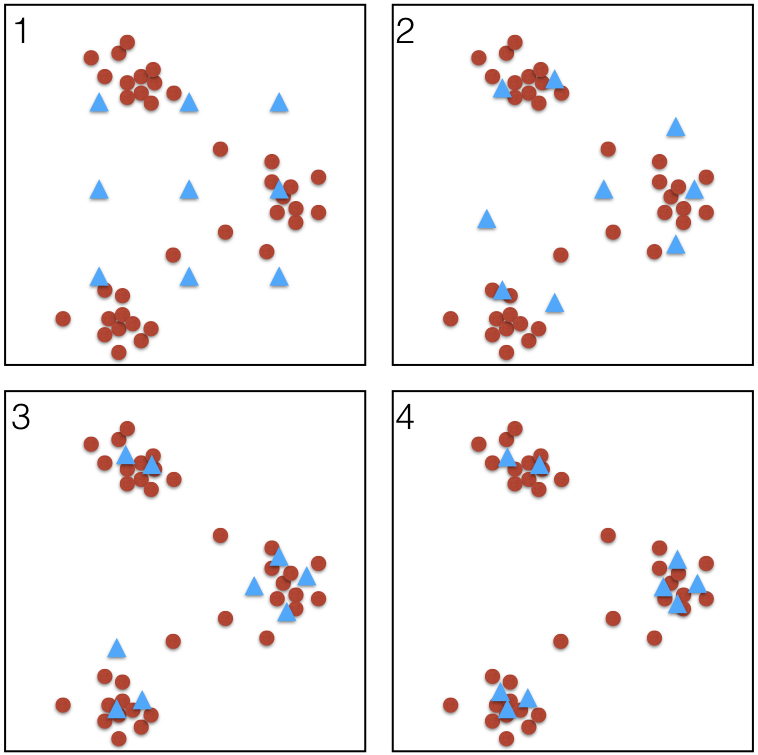
\includegraphics[width=0.95\columnwidth]{sofm_fitting.png}
	\caption{
		Schematic illustration of the clustering problem considered in this paper.  
		Blue triangles represent clusters and red dots are data points. 
		The training process moves clusters to fit the data points. 
		Note that there are fewer clusters than data points, 
		which is the essence of dimensionality reduction, 
		and is what permits the model to generalize the data.
	}
	\label{fig:sofm_fitting}
\end{figure}


























\section{The quantum assisted self-organizing feature map (QASOFM)}
\label{sec:qasofm}



\subsection{The classical algorithm}


The SOFM is one of the most widely-used unsupervised learning methods used in various areas of modern science. 
It was first proposed by Kohonen as a self-organizing unsupervised learning algorithm which produces feature maps similar to those occurring in the brain \cite{solan2001}. 
The SOFM algorithm operates with a set of input objects, each represented by a $N$-dimensional vector, 
and describes a mapping from a higher-dimensional input space to a lower-dimensional map space that preserve the topological properties of the input space, commonly a bi-dimensional map.

The input dimensions are associated with the features, 
and the nodes in the grid (called cluster vectors) are assigned the $N$-dimensional vectors. 
The components of these vectors are usually called weights. 
Initially the weight components are chosen randomly. 
We then can train our SOFM adjusting the components through the learning process which occur in the two basic procedures of 
selecting a winning cluster vector, also called the best matching unit, and updating its weights (Fig.~\ref{fig:sofm_fitting}). 
More specifically, they consist of four step process: 
\begin{enumerate*}
\item selecting an input vector randomly from the set of all input vectors; 
\item finding a cluster vector which is closest to the input vector; 
\item adjusting the weights of the best matching unit and neurons close to it on feature map in such a way 
	that these vectors  becomes even closer to the input vector; 
\item repeating this process for many iterations until it converges.
\end{enumerate*}


On a step $t$ when the best matching unit $\vec{w}_{c}$ for a input $\vec{x}(t)$ is selected, 
the weights $\vec{w}_{i}$ of the best matching unit and its neighbors on feature map are adjusted according to
%
\begin{equation}
    \label{eq:learning}
	\vec{w}_{i}(t + 1) 
	= \vec{w}_{i}(t)
	+ \theta(c, i, t) \alpha(t) 
		\left(\vec{x}(t) - \vec{w}_{i}(t)\right) ,
\end{equation}
%
where  $\alpha(t)$ is the monotonically decreasing learning rate and $\theta(c, i, t)$ is the neighborhood function (usually Gaussian, Delta or the mexican-hat function) which defines the vicinity of the BMU noted by index $c$ in which the weights also should be adjusted and depends on distance on feature map. This expression can be interpreted according to: if a component of the input vector $\vec{x}(t)$ is greater than the corresponding weight $ \vec{w}_{i}(t) $, increase the weight of the BMU and the weights indexed by $i$ and defined with the neighborhood function by a small amount defined by the learning rate $\alpha(t)$; if the input component is smaller than the weight, decrease the weight by a small amount. The larger the difference between the input component and the weight component, the larger the increment (decrement). 

Intuitively, this procedure can be geometrically interpreted as iteratively moving the cluster vectors defined by the corresponding weight $ \vec{w}_{i}(t) $ (blue triangles on Fig.~\ref{fig:sofm_fitting}) in space one at a time in a way that ensures each move is following the current trends inferred from their distances to the input objects defined by $\vec{x}(t)$ (red dots on Fig.~\ref{fig:sofm_fitting}). A visualisation of this process is shown in Fig.~\ref{fig:sofm_fitting}.

In the original version of SOFM, the winning cluster vector was selected based on the Euclidean distance between an input vector and the cluster vectors. In this paper we deal with binary vectors clustering problem and for binary data the Hamming distance is more suitable \cite{appiah2009, santana2017}.
Using a simple technique of encoding classical binary information into a quantum register \cite{trugenberger2001},
we introduce an optimized algorithm for calculating the matrix of Hamming distances between all input and cluster vectors at once.







\subsection{Optimized quantum scheme for Hamming distance calculation}
\label{subsec:qcircuit}


%%%%%
\begin{figure}[t]
	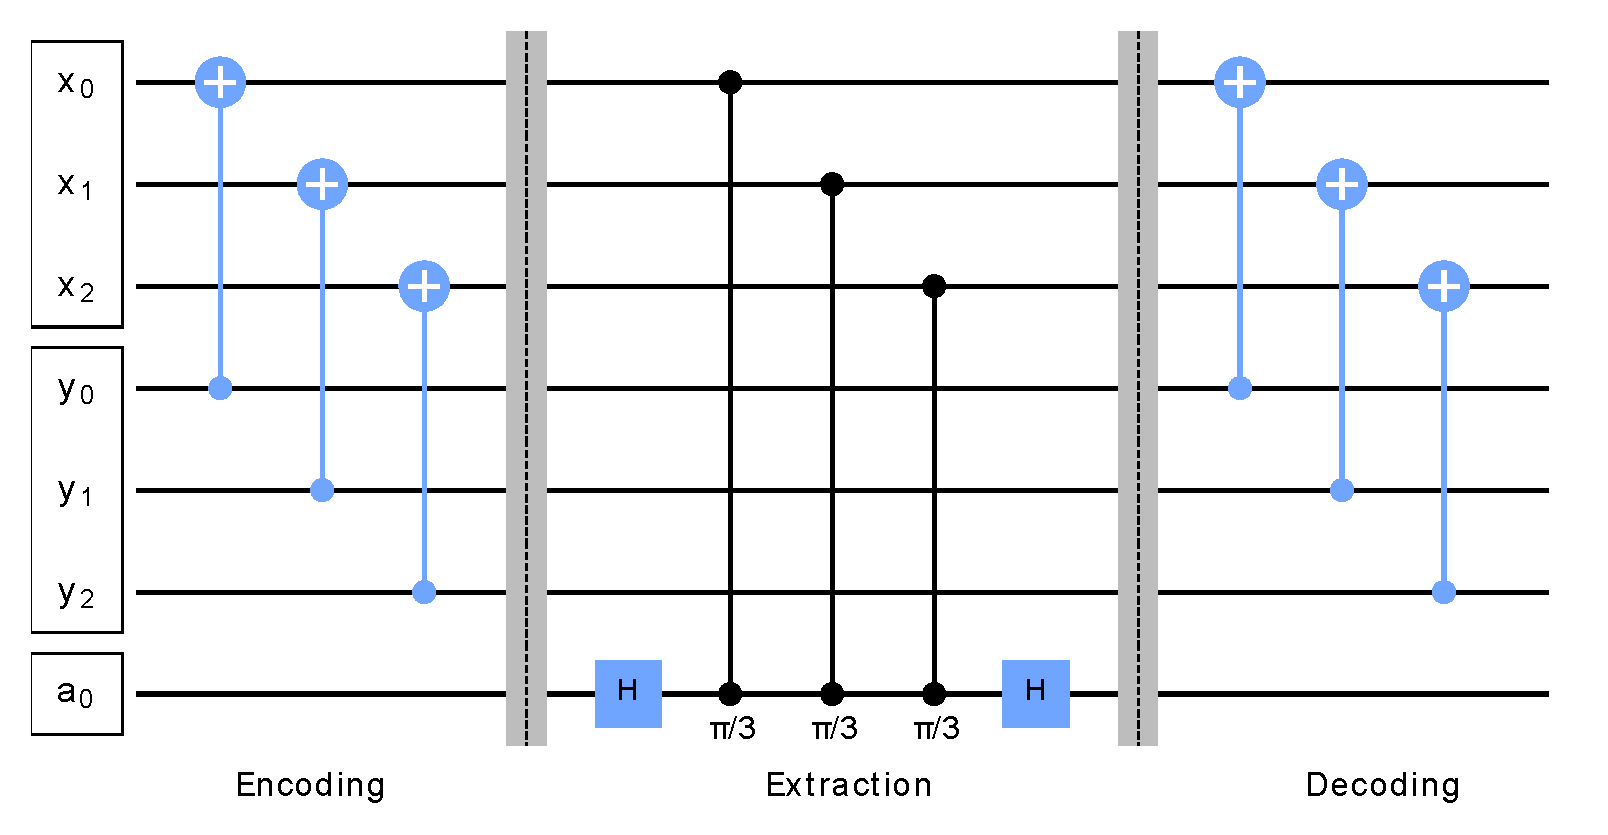
\includegraphics[width=\columnwidth]{qcircuit.eps}
	\caption{ \hl{Iliya, could you please change the picture to the case with the controlled phase gate and make correction of the caption in appropriate way}
		Quantum circuit for the quantum parallelized Hamming distance calculating  between all pairs of binary vectors from two sets ${X}$ and ${Y}$ encoded in $X$ and $Y$ quantum registers   respectively.
		First, we encoded information about pairwise different qubits in a quantum state of the $X$-register with applying the CNOT gates. 
		Second, Hamming distance values are extracted into the amplitudes of superposition with the controled rotation around $z$-axis gate(see Eq.~(\ref{eq:controled_rotation})) and Hadamard gates. 
		Finally, a quantum state of the $X$-register returned to the initial basis for information retrieval. 	
	} 
	\label{fig:qcircuit}
\end{figure}
%%%%%



%%%%%
\begin{figure}[t]
	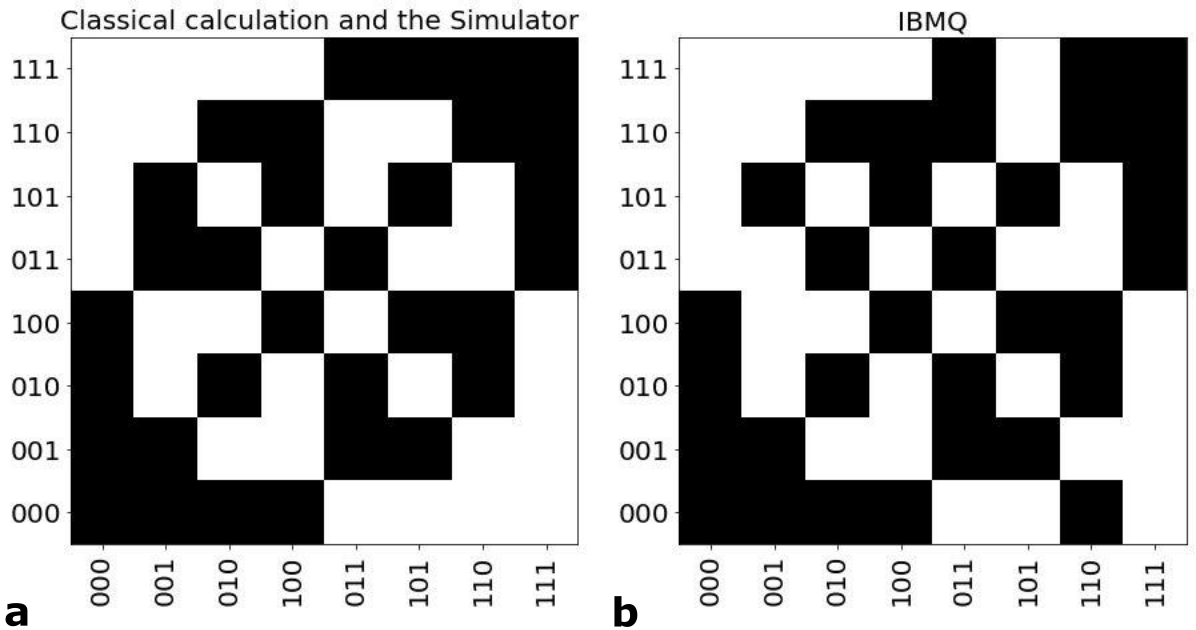
\includegraphics[width=0.95\columnwidth]{distance_matrix.png}
	\caption{\hl{[AP: Iliya, could you please recalculate the fidelity for this picture it looks that it is even higher for thee picture because there is basically less red crosses and rewrite the caption in the appropriate way]}
		Hamming distance matrix between two data sets of binary vectors. 
		Values of distance that less than median distance value was marked black. The classical simulation of the quantum circuit shows perfect agreement to theoretical calculations and presented on the left figure. Result obtained on  IBMQ "ibmq\_16\_melbourne" backend is shown on the right figure.
		Result obtained on the IBM Q Experience ``ibmq\_16\_melbourne'' backend. 
		Fidelity of final state~(\ref{eq:final_state}) measurement is 0.8.}
	}
	\label{fig:distance_matrix}
\end{figure}
%%%%%





The overall procedure involves two registers of $n$ qubits each, denoted $\left| X \right\rangle$ and $\left| Y \right\rangle$, along with a single auxiliary qubit $\left| a \right\rangle$. 
During the whole process, the $\left| Y \right\rangle$ register is used to store the cluster states.  
At the beginning and end of the procedure, the $\left| X \right\rangle$ register stores the input vectors.  
During the procedure it stores the differences between input vectors and cluster states.

Let us assume we have $N_x$ input vectors and $N_y$ cluster states. 
The $i$th input vector and $j$th cluster vector are respectively denoted as $\left| x_i \right\rangle$, $\left| y_j \right\rangle$. 
The registers $\left| X \right\rangle$ and $\left| Y \right\rangle$ are initialized to store the input vectors and cluster vectors according to
%
\begin{align}
    \label{eq:encodnig}
    \left| X \right\rangle  & = \frac{1}{\sqrt{N_x}} \sum\limits_{i=1}^{N_x} \left| x_i \right\rangle,  \\
    \left| Y \right\rangle&  = \frac{1}{\sqrt{N_y}} \sum\limits_{j=1}^{N_y} \left| y_j \right\rangle .
\end{align}
% 
The two registers along with the auxiliary qubit comprise the initial state of the quantum computer according to
%
\begin{equation} 
    \label{eq:initial_state}
	\left| \psi_0 \right\rangle = 
    \left| X \right\rangle
    \left| Y \right\rangle 
    \left| a \right\rangle ,
\end{equation}
%
where $\left| a \right\rangle$ is an auxiliary qubit in the state $\left| 0 \right\rangle$ initially.

Given this initial state we may begin the processing of the problem.  The quantum circuit that we follow is shown in Fig.\ref{fig:qcircuit}. We start by elementwise applying CNOT gates between all the qubits of the X and Y registers (the "Encoding" part of Fig. \ref{fig:qcircuit}) $\left| x^{(\alpha)} y^{(\alpha)} \right\rangle$ 

\begin{equation}
    | \psi_1 \rangle  =  
    \frac{1}{\sqrt{N_x N_y}} \sum_{i, j=1}^{N_x,N_y} 
    | d^{(1)}_{ij}, \dots, d^{(n)}_{ij} \rangle 
    | y^{(1)}_j, \dots, y^{(n)}_j \rangle
    | 0 \rangle ,
\end{equation}
%
where $d^{(\alpha)}_{ij} = \mathrm{CNOT}(y^{(\alpha)}_i, x^{(\alpha)}_j)$, and $\alpha = 1 \dots n$  is the qubit index in the register. 
At this stage of the computation the $\left| X \right\rangle$ no longer stores the input vectors,
instead it stores the information about pairwise different qubits between the input vectors $\left| x_i \right\rangle$ and cluster vector $\left| y_j \right\rangle$. 

The next step, depicted on the Fig.\ref{fig:qcircuit} as the "Extraction" stage, is to extract the accumulated information about the differences between each pair $\left| x_i \right\rangle$ and $\left| y_j \right\rangle$ by projection onto the amplitude of the superposed state. This is achieved by applying the Hadamard gate on auxiliary qubit, followed by a controlled phase gate on $\left|a\right\rangle \left|d_{ij}^{(\alpha)}\right\rangle$ 
%~(\ref{eq:control_phase_rotation})
\begin{equation}
    \label{eq:control_phase_rotation}
    R_{(X,a)}(\phi) = 
    \begin{pmatrix}
        1 & 0 & 0 & 0 \\
        0 & 1 & 0 & 0 \\
        0 & 0 & 1 & 0 \\
        0 & 0 & 0 & e^{-i\phi}
    \end{pmatrix} ,
    \quad \phi = \frac{\pi}{n}
\end{equation}
%
where $d_{ij}^{(\alpha)}$ is the control qubit and the ancilla qubit $\left| a \right\rangle$ is the target. Finally, another Hadamard gate is applied on the ancilla qubit (see Fig.~\ref{fig:qcircuit}). 

After the first Hadamard on the ancilla qubit the state is
%
\begin{equation}
    \left| \psi_2 \right\rangle = 
    \frac{1}{\sqrt{N_x N_y}}\sum\limits_{i, j=1}^{N_x,N_y} 
    \left| d_{ij} \right\rangle 
    \left| y_j \right\rangle
    \dfrac{(\left| 0 \right\rangle + \left| 1 \right\rangle)}{\sqrt{2}},
\end{equation}
%
where $\left| d_{ij} \right\rangle = \left| d_{ij}^{(1)},\ldots,d_{ij}^{(n)} \right\rangle$.
Applying the controlled phase gate on $\left| x^{(\alpha)} a \right\rangle$ where $\alpha = 1\dots n$ and the state then becomes
%
\begin{multline}
    \left| \psi_3 \right\rangle = R_{(X,a)}\left(\dfrac{\pi}{n}\right)\left| \psi_2 \right\rangle
    \\ = \dfrac{1}{\sqrt{2 N_x N_y}}
				\sum\limits_{i, j=1}^{N_x,N_y} 
				\left| d_{ij} \right\rangle 
        \left| y_j \right\rangle 
        \left| 0 \right\rangle
        \\ + \dfrac{1}{\sqrt{2 N_x N_y}}
				\sum\limits_{i, j=1}^{N_x,N_y}
        \exp\left(\dfrac{-i \pi}{n}\sum\limits_{l=1}^n d^{(l)}_{ij} \right)
        \left| d_{ij} \right\rangle 
\\ \times        \left| y_j \right\rangle 
        \left| 1 \right\rangle
\end{multline}
%
Applying another Hadamard on the ancilla qubit we obtain
%
\begin{multline}
    \left| \psi_4 \right\rangle = 
    \frac{1}{\sqrt{N_x N_y}}\sum\limits_{i, j=1}^{N_x,N_y} 
    \exp \left(\dfrac{-i \pi}{2n}\sum\limits_{l=1}^n d^{(l)}_{ij} \right)
		\\ \times
        \left[ \cos\left(\dfrac{\pi}{2n}\sum\limits_{l=1}^n d^{(l)}_{ij} \right)
        \left| d_{ij} \right\rangle 
        \left| y_j \right\rangle 
        \left| 0 \right\rangle\right.
        \\+ 
        \left. i \sin\left(\dfrac{\pi}{2n}\sum\limits_{l=1}^n d^{(l)}_{ij} \right)
        \left| d_{ij} \right\rangle 
        \left| y_j \right\rangle 
        \left| 1 \right\rangle\right] .
\end{multline}
%
This completes the step for projecting differences between pairs of $\left| x_i \right\rangle$ and $\left| y_j \right\rangle$ onto the amplitude of the auxiliary qubit. 
The process is done in the $x$-basis, achieved by the surrounding Hadamard gates. 
There are two possible measurement outcomes of the auxiliary qubit.  
Each pair of $\left|x_i \right\rangle$ and $\left| y_j \right\rangle$ forms a subspace of the Hilbert space, 
the controlled phase gate ensures to change amplitudes of those outcomes within this subspace depending on how different the spin configurations between $\left| x_i \right\rangle$ and $\left| y_j \right\rangle$ are.

At this stage, the information regarding the differences between pairs of $\left| x_i \right\rangle$ and $\left| y_j \right\rangle$ encoded in the amplitudes, in order to extract the Hamming distances between the relevant $\left| x_i \right\rangle$, $\left| y_j \right\rangle$ we return to our initial basis for register $\left| X \right\rangle$ by applying pairwise CNOT gates:
%
\begin{multline}
		\label{eq:final_state}
    \left| \psi_f \right\rangle = 
    \mathrm{CNOT} (Y,X)\left| \psi_4 \right\rangle \\=  
    \sum\limits_{i, j=1}^{N_x,N_y} 
    \exp \left(\dfrac{-i \pi}{2n}\sum\limits_{l=1}^n d^{(l)}_{ij} \right)
				\left[ \cos\left(\dfrac{\pi}{2n}\sum\limits_{l=1}^n d^{(l)}_{ij} \right)
        \left| x_i \right\rangle 
        \left| y_j \right\rangle 
        \left| 0 \right\rangle\right.
        \\+
        \left. i \sin\left(\dfrac{\pi}{2n}\sum\limits_{l=1}^n d^{(l)}_{ij} \right)
        \left| x_i \right\rangle 
        \left| y_j \right\rangle 
        \left| 1 \right\rangle\right] .
\end{multline}
%
Thus we return int the initial basis and the amplitudes of the auxiliary qubit are proportional to how different each pairs of $\left| x_i \right\rangle$ and $\left| y_j \right\rangle$ are.

From the statistics of the measurement outcomes of final state~(\ref{eq:final_state}) we recreate the amplitudes of ancilla qubit states. 
From those amplitudes estimations we are able to plot the distance matrix between two data sets of binary vectors.
The probability amplitude of the ancilla qubit outcomes captures the exact Hamming distance as the result of the preprocessing function.
There are two possible outcomes of measurement of the ancilla qubit, each has its probability amplitude and own interpretation of that amplitude. 
For instance, for the $\left| 0 \right\rangle$ outcome, the larger the amplitude the smaller the Hamming distance, 
and for the $\left| 1 \right\rangle$ outcome it is the other way around, the magnitude of the amplitude of that outcome is proportional to the Hamming distance.

Measuring the Hamming distance of a particular pair of input vectors $\left| x_i \right\rangle$ and cluster vectors $\left| y_j \right\rangle$ consists of extracting the relevant amplitude from the subspace that those states form, 
this can be done using the following projection operator
%
\begin{align}
\Pi_{i,j} = &\left| x_i \rangle\langle x_i \right| \otimes \left| y_j \rangle\langle y_j \right| \otimes I .
\end{align} 
%
Using the above projection operator, the subspace of the Hilbert space formed by a particular pair of input and cluster vectors can be traced out as
%
\begin{align}
    \rho_{i,j} &= \text{Tr}_{X,Y} (\Pi_{i,j} \left| \psi_f \rangle\langle \psi_f \right| \Pi_{i,j}) .
\end{align}
%
From the reduced density matrix, the following two amplitudes for the measurement results can be extracted
%
\begin{align}
    a_0(x_i,y_j) & = \frac{\left\langle 0 |\rho_{i,j}| 0 \right\rangle}{\text{Tr}(\rho_{i,j})}  \\
    a_1(x_i,y_j) & = \frac{\left\langle 1 |\rho_{i,j}| 1 \right\rangle}{\text{Tr}(\rho_{i,j})} .
\end{align}
%
Currently available quantum platforms are still subject to substantial level of noise and extracting the exact distance from amplitude is still a difficult task. In order to reduce noise we average the measurement results over different states of the ancillary qubit, thus the measured Hamming distance between the input vector $\left| x_i \right\rangle$ and cluster vector $\left| y_j \right\rangle$ is
%
\begin{align}
    d_{i,j}^H & \propto 1 - \frac{1}{2}(a_0(x_i,y_j) + (1-a_1(x_i,y_j))) .
\end{align}
%
The Hamming distance measured in this way is bounded $0 \leq d_{i,j}^H \leq 1$, 
where  $0$ indicates that $x_i$ are $y_j$ identical and $1$ means they are completely opposite in terms of their pairwise binary coordinates.

The number of controlled gate operations to define the full distance matrix matches the number of controlled gate operations in \cite{trugenberger2001}, where the original algorithm for calculation of the Humming distance was introduced, but the number of remaining gates is reduced compared to \cite{trugenberger2001}, leading to less deep circuit, which is significant for NISQ devices.


%In this special case scenario the circuit depth complexity is matching with \cite{schuld2014}.

  


%%%%%
\begin{figure}[t]
	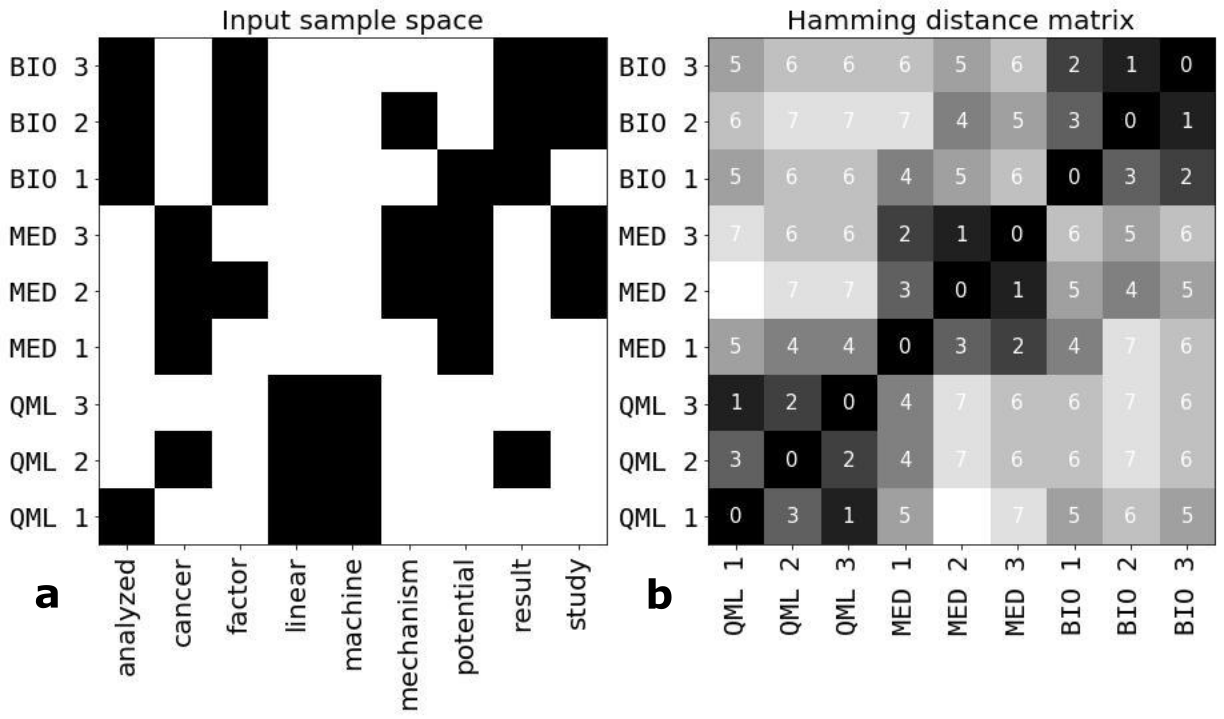
\includegraphics[width=0.95\columnwidth]{vectorized_sample.png}
	\caption{
		(a) Representation of the data set of abstracts with the bag-of-words \cite{weikang2016} model is shown. 
		Each abstract is represented by a binary vector with 9 elements, corresponding to the 9 words on the horizontal axis. 
		The samples are sorted into groups ``Quantum Machine Learning'' (QML), ``Cancer'' (MED) and ``Gene Expression'' (BIO) with 3 papers for each tag, for a total of 9 paper.    
		(b) The Hamming distance between each vectorized abstract is shown as a number in the matrix. 
	} 
	\label{fig:vectorized_sample}
\end{figure}
%%%%%



















\section{Experimental demonstration of QASOFM}

We now show experimental results for a proof-of-concept demonstration of the algorithm introduced in the previous section, on a 16-qubit quantum computer provided by IBM Q Experience.  
We perform unsupervised data clustering for three sets of paper abstracts from three different fields: 
quantum physics \cite{qml0, qml1, qml2}, 
medicine \cite{med0, med1, med2} 
and biology \cite{bio0, bio1, bio2}. 
Each set consists of three papers selected at random that focus on one of following topics: 
``Quantum Machine Learning'', 
``Cancer'' 
and ``Gene Expression''. 
Abstracts were vectorized by the bag-of-words \cite{weikang2016} model in order to choose the most defining words in each data set (see Fig.~\ref{fig:vectorized_sample}) \cite{mctear2016}.  
This model represents text as a multiset ``bag'' of its words taking into account only the multiplicity of words. 
Preparing the bag-of-words we excluded the words that appear only in one abstract and more than in 4 abstracts and we also excluded the word ``level'' from consideration due to the frequent overlap between the clusters because it gives instabilities for both classical and quantum algorithms. 
We restricted our bag-of-word size to 9 of the most frequent words from the full bags-of-word  due to limitations on the number of qubits. 
After vectorizing and pre-processing  the data, the clusters are well-separated with the Hamming distance.  
We observe that distances between the abstracts inside clusters are smaller than distances between the abstracts from different clusters, 
showing successful self-organization (Fig.~\ref{fig:vectorized_sample}). 


In classical SOFM \cite{kohonen1990}, first a distance calculation between a sample vector and all cluster vectors is made, 
then the closest cluster vector is shifted towards the sample vector. 
The complexity of algorithm, in the sense of the number of distance calculations, scales as $O(LMN)$, 
where $N$ is number of samples, 
$M$ is number of randomly sampled cluster vectors, 
and $L$ is number of the shifts of cluster vectors.  
In the QASOFM described in the previous section, distance calculations are realized on a quantum device (i.e. the IBM Q Experience) with the use of circuit presented in Fig.~\ref{fig:qcircuit}. This approach allows one to reduce the number of operations in a number of cluster states with an optimized number of gates 
that are possible to realize on  quantum computing devices that are currently available. 
The circuit realized in this way such 
that the calculation of Hamming distance implemented step-by-step between each sample vector and all cluster vectors is realized in one operation. In this case, as there is only one input vector considered, the ``Decoding'' stage (Fig.~\ref{fig:qcircuit}) can be removed as measurement no longer needs to indicate for which input vector the distance has been measured.
The complexity of the quantum assisted SOFM then scales as $O(LN)$. 

In order to check that our algorithm gives the expected results we compare it to classical calculations of the distance matrix on two data sets of binary vectors, as shown in Fig.~\ref{fig:distance_matrix}.  
We see good agreement between the distance matrices calculated classically and on the IBM Q Experience. 
The match is close, but not perfect, and we attribute it to noise in the currently available non fault-tolerant quantum processors.

An example of the QASOFM learning process is shown in Fig.~\ref{convergence}. 
Initially, the cluster vectors were randomly chosen and the label of sample distribution is shown for the zeroth epoch in Fig.~\ref{convergence}(a). In order to prepare a superposition of cluster vectors needed for the calculation of the distance matrix we use the standard initialization of QISKIT\cite{qiskit} library. 
Each epoch of the algorithm consists of distance calculation between all data and cluster vectors 
and requires 9 distance calculations in the  quantum implementation ($N$ in general case) 
or 27 distance calculations for classical realization 
($MN$ in general case). 
After the distance calculation from each sample to all cluster vectors at each epoch we label each sample with the index of the closest cluster vector 
and shift the closest cluster vectors to the sample one. 
The shift is made by the change of the first binary element in the cluster vectors different from the sample one. 
The evolution of the labels presented on Fig.~\ref{convergence}(c).  
Good convergence is already observed in the fourth epoch.

This proof of concept example shows that developing of noisy intermediate scale quantum hardware will allow to solve some practical problems in unsupervised manner with very simple encoding of categorical data to quantum register. 
Furthermore, it shows that it is possible to develop distance based hybrid quantum classical algorithms 
that speed up classical counterparts and can be implemented on near future quantum devices 
and that further developing distance based hybrid algorithms, 
that can learn in unsupervised manner, for categorical data such as genomic and so on has significant interest.

%%%%%
\begin{figure}[t]
	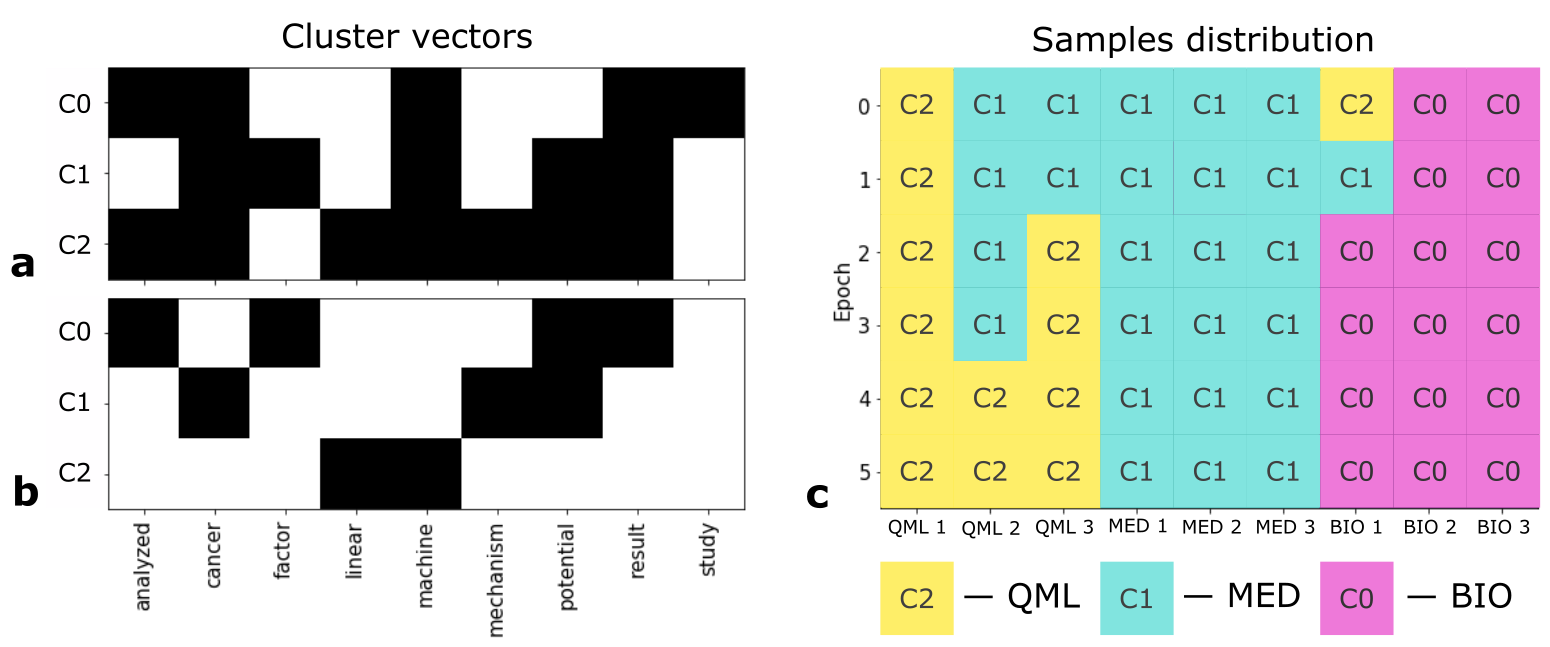
\includegraphics[width=0.95\columnwidth]{convergence.png}
	\caption{
		(a) Initial random binary vectors of cluster vectors (labeled as C0, C1, C2), 
		for the selected 9 words from the bag of words model. 
		(b) The result of applying our QASOFM implemented on the IBM Q Experience simulator backend. 
		Vectors mean cluster elements for BIO, MED, QML groups, 
		for the C0, C1, C2 cluster vectors, respectively. 
		(c) The evolution of label distribution on each learning epoch.
	} 
	\label{convergence}
\end{figure}
%%%%%



\section{Discussions}
We have developed a quantum assisted SOFM and showed a proof-of-concept experimental demonstration 
that it can be used to solve clustering problems in an unsupervised manner.  
The procedure of solving such clustering problem requires calculating the distance many times in iterative way, 
which is calculated using a hybrid quantum-classical procedure.  
We introduced an optimized circuit for Hamming distance calculations that can be implemented on currently available quantum computing devices with high fidelity. 
Our quantum circuit performs the distance-computing component of a classical SOFMs algorithm 
and in this way improve its performance. 
The complexity of the quantum assisted SOFM scales as $O(LN)$ 
while the complexity of the fully classical SOFM scales as $O(LMN)$, 
where $N$ is number of samples, $M$ is number of randomly sampled cluster vectors, 
and $L$ is number of the shifts of cluster vectors.
Due to wide use of classical SOFMs in different areas of modern research and technology, 
this can give opportunities for the use of QASOFM in practical applications in near term, outperforming classical algorithms. 
In addition, as our algorithm performs the Hamming distance calculation, 
it has the potential to enhance any classical algorithm that relies on calculating distances between data entries of vector form. 
In machine learning, data science, statistics and optimization, distance is a common way of representing similarity, calculating it between large data sets is common procedure 
and our circuit could potentially enhance other distance-based algorithms as long as exact distance is not required, 
but when knowledge of nearest vectors is sufficient.



\section*{Acknowledgments}
The work is supported by the RFBR-NSFC collaborative program (Grant No. 18-57-53007) and the State assignment (N. 0089-2019-0002). I.D.L. acknowledges support from the Russian Foundation for Basic Research, grant No.19-32-80004 and support from the Foundation for the Advancement of Theoretical Physics and Mathematics “BASIS” No.19-1-5-130-1. T.B. is supported by the Shanghai Research Challenge Fund; New York University Global Seed Grants for Collaborative Research; National Natural Science Foundation of China (61571301, D1210036A); the NSFC Research Fund for International Young Scientists (11650110425, 11850410426); NYU-ECNU Institute of Physics at NYU Shanghai; the Science and Technology Commission of Shanghai Municipality (17ZR1443600); the China Science and Technology Exchange Center (NGA-16-001); and the NSFC-RFBR Collaborative grant (81811530112).





%\section*{Author Contributions}

%I.D.L. and A.N.P. performed the calculations. All authors discussed the results and wrote the paper. 





\section*{Conflict of interest}

The authors declare no conflict of interest.


\section*{Keywords}
quantum self-organizing feature map; quantum machine learning; neural network; quantum unsupervised data clustering; Hamming distance.

\bibliographystyle{naturemag}
\bibliography{bibliography}

\end{document}
